% This file was created by tikzplotlib v0.9.8.
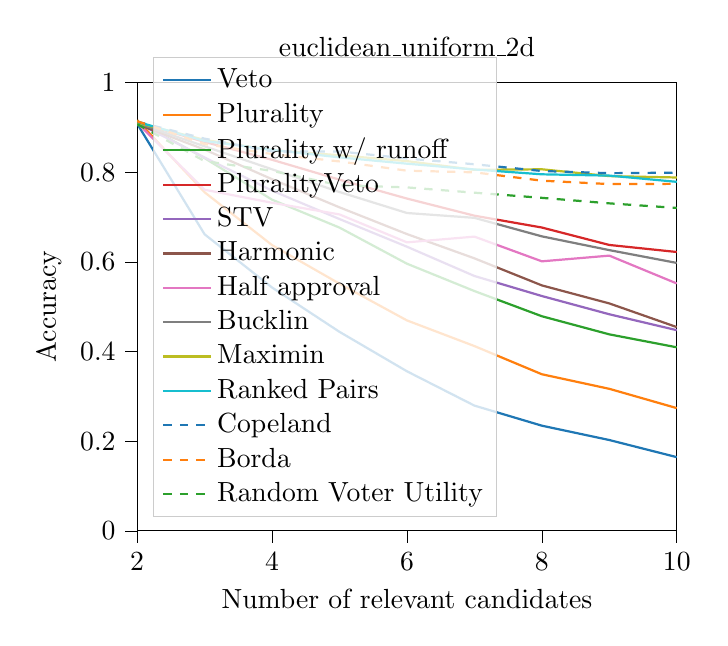
\begin{tikzpicture}

\definecolor{color0}{rgb}{0.12156862745098,0.466666666666667,0.705882352941177}
\definecolor{color1}{rgb}{1,0.498039215686275,0.0549019607843137}
\definecolor{color2}{rgb}{0.172549019607843,0.627450980392157,0.172549019607843}
\definecolor{color3}{rgb}{0.83921568627451,0.152941176470588,0.156862745098039}
\definecolor{color4}{rgb}{0.580392156862745,0.403921568627451,0.741176470588235}
\definecolor{color5}{rgb}{0.549019607843137,0.337254901960784,0.294117647058824}
\definecolor{color6}{rgb}{0.890196078431372,0.466666666666667,0.76078431372549}
\definecolor{color7}{rgb}{0.737254901960784,0.741176470588235,0.133333333333333}
\definecolor{color8}{rgb}{0.0901960784313725,0.745098039215686,0.811764705882353}

\begin{axis}[
legend cell align={left},
legend style={
  fill opacity=0.8,
  draw opacity=1,
  text opacity=1,
  at={(0.03,0.03)},
  anchor=south west,
  draw=white!80!black
},
tick align=outside,
tick pos=left,
title={euclidean\_uniform\_2d},
x grid style={white!69.0196078431373!black},
xlabel={Number of relevant candidates},
xmin=2, xmax=10,
xtick style={color=black},
y grid style={white!69.0196078431373!black},
ylabel={Accuracy},
ymin=0, ymax=1,
ytick style={color=black}
]
\addplot [thick, color0]
table {%
2 0.9081
3 0.6614
4 0.5427
5 0.4438
6 0.3558
7 0.2793
8 0.2345
9 0.2025
10 0.1643
};
\addlegendentry{Veto}
\addplot [thick, color1]
table {%
2 0.916
3 0.7551
4 0.6373
5 0.5512
6 0.4693
7 0.4121
8 0.3492
9 0.3167
10 0.2737
};
\addlegendentry{Plurality}
\addplot [thick, color2]
table {%
2 0.9137
3 0.8313
4 0.7386
5 0.6763
6 0.5958
7 0.5348
8 0.4786
9 0.4382
10 0.4093
};
\addlegendentry{Plurality w/ runoff}
\addplot [thick, color3]
table {%
2 0.9114
3 0.8675
4 0.8276
5 0.7832
6 0.7411
7 0.7029
8 0.6765
9 0.6376
10 0.6219
};
\addlegendentry{PluralityVeto}
\addplot [thick, color4]
table {%
2 0.9102
3 0.8327
4 0.7588
5 0.6954
6 0.6337
7 0.5684
8 0.5237
9 0.483
10 0.4475
};
\addlegendentry{STV}
\addplot [thick, color5]
table {%
2 0.9072
3 0.8504
4 0.7843
5 0.7215
6 0.6619
7 0.6078
8 0.5474
9 0.5072
10 0.4544
};
\addlegendentry{Harmonic}
\addplot [thick, color6]
table {%
2 0.91
3 0.7608
4 0.7317
5 0.7057
6 0.6434
7 0.6562
8 0.6011
9 0.6138
10 0.5517
};
\addlegendentry{Half approval}
\addplot [thick, white!49.8039215686275!black]
table {%
2 0.9094
3 0.8576
4 0.8064
5 0.7557
6 0.7089
7 0.6981
8 0.6568
9 0.6261
10 0.5975
};
\addlegendentry{Bucklin}
\addplot [thick, color7]
table {%
2 0.9101
3 0.872
4 0.8489
5 0.8377
6 0.8246
7 0.8052
8 0.8064
9 0.7912
10 0.7881
};
\addlegendentry{Maximin}
\addplot [thick, color8]
table {%
2 0.9123
3 0.8695
4 0.8497
5 0.833
6 0.8189
7 0.806
8 0.7952
9 0.7923
10 0.7784
};
\addlegendentry{Ranked Pairs}
\addplot [thick, color0, dashed]
table {%
2 0.9125
3 0.8747
4 0.8462
5 0.8463
6 0.8304
7 0.8176
8 0.8026
9 0.7977
10 0.7989
};
\addlegendentry{Copeland}
\addplot [thick, color1, dashed]
table {%
2 0.9136
3 0.8626
4 0.8404
5 0.8239
6 0.8033
7 0.7996
8 0.781
9 0.7734
10 0.7739
};
\addlegendentry{Borda}
\addplot [thick, color2, dashed]
table {%
2 0.907
3 0.8246
4 0.8028
5 0.7708
6 0.766
7 0.7542
8 0.7427
9 0.7304
10 0.7202
};
\addlegendentry{Random Voter Utility}
\end{axis}

\end{tikzpicture}
